% !TeX program = xelatex
\documentclass[11pt]{article}

\usepackage[a4paper,margin=25mm]{geometry}
\usepackage{fontspec}
\usepackage{xeCJK}
\setmainfont{TeX Gyre Termes}
\setsansfont{TeX Gyre Heros}
\setmonofont{Latin Modern Mono}
\setCJKmainfont[BoldFont=SimHei]{SimSun}
\setCJKsansfont{SimHei}
\setCJKmonofont{SimSun}

\usepackage{amsmath,amssymb,amsthm,bm,mathtools}
\usepackage{booktabs,tabularx,array,longtable,multirow}
\usepackage{graphicx}
\usepackage{caption}
\usepackage{subcaption}
\usepackage{xcolor}
\usepackage{enumitem}
\usepackage{microtype}
\usepackage{natbib}
\usepackage{xurl}
\usepackage{hyperref}
\usepackage[nameinlink,noabbrev]{cleveref}
\usepackage{placeins}

\hypersetup{
  colorlinks=true,
  linkcolor=blue!55!black,
  citecolor=green!35!black,
  urlcolor=blue!60!black,
  pdftitle={Filtration-Coherent and Exchange-Equivariant World Cup Forecasting},
  pdfauthor={Anonymous Research Team}
}
\graphicspath{{figures/}}
\captionsetup{font=small,labelfont=bf}
\setlist{nosep,leftmargin=*}
\setlength{\parskip}{0.35em}
\setlength{\parindent}{1.5em}
\setlength{\emergencystretch}{2em}
\raggedbottom
\newcolumntype{Y}{>{\raggedright\arraybackslash}X}

\newtheorem{proposition}{Proposition}
\newtheorem{remark}{Remark}
\newcommand{\Fpre}{\mathcal F^{\mathrm{pre}}}
\newcommand{\Fkick}{\mathcal F^{\mathrm{kickoff}}}
\newcommand{\Fht}{\mathcal F^{\mathrm{HT}}}
\newcommand{\KL}{D_{\mathrm{KL}}}
\newcommand{\AZero}{\mathrm{A0}}

\title{\textbf{Filtration-Coherent and Exchange-Equivariant World Cup Forecasting under Edition Shift}\\
\large Development Validation, a One-Shot 2014 Audit, and an Official-Format 2026 Scenario}
\author{Anonymous Research Team}
\date{Final evidence audit 18 July 2026}

\begin{document}
\maketitle

\begin{abstract}
World Cup forecasting combines sparse tournament environments, changing institutions, neutral
venues, partially observed personnel, and multiple outputs that should arise from one probability
law.  We construct an auditable study around an information filtration, an $S_2$ team-exchange
action, a penalized attack--defence count model, and a coherent finite score grid.  Three estimands
are kept separate.  First, seven expanding-origin development folds (1986--2010; 412 OOF matches)
select and calibrate the model.  Relative to frozen Dixon--Coles, equal-edition WDL log loss improves
by $0.0204$ (95\% edition-bootstrap interval $[0.0035,0.0365]$) and Brier by $0.0130$
($[0.0027,0.0237]$), with five wins in seven folds.  Second, a batch-blind realized-fixture audit
seals all 64 sets of 2014 predictions before one target read.  It does not reproduce the development
advantage: advanced calibrated log loss/Brier are $1.0227/0.6090$, versus $0.9851/0.5876$ for the
frozen Dixon--Coles baseline.  Selection is not reopened.  A separate cost-sensitive action layer
recovers draw recall $0.3846$ but is not a proper-score model.  Third, an official Annex C/M73--M104
engine runs 220,000 illustrative 2026-format tournaments under historical profile stand-ins,
stopping at the preregistered MCSE gate; expected tournament goals are $181.165$ (MCSE $0.0287$).
The associated sensitivity decomposition attributes 55.0\%, 24.5\%, and 20.5\% of total-goal
variance to parameter, scoring-regime, and path-plus-match components.  These are scenario
quantities, not factual entrant forecasts or future coverage guarantees.  The contribution is a
falsifiable evidence chain that retains adverse external results and structural failures, not a
claim of universal predictive superiority.
\end{abstract}

\begin{center}
\begin{minipage}{0.95\linewidth}
\textbf{中文摘要。}
世界杯预测同时面临样本稀疏、制度迁移和多输出一致性。本文将三类估计量严格分离：第一，
1986--2010年七届扩展起点外层验证用于模型选择；校准模型相对冻结的Dixon--Coles基线，
胜平负log loss和Brier的等届平均改善分别为0.0204和0.0130，并在5/7届获胜。第二，2014年
一次性审计先封存64场比赛的胜平负与联合比分分布，随后只读取一次标签。外部结果未复现开发期
优势：高级模型的log loss/Brier为1.0227/0.6090，弱于基线的0.9851/0.5876；模型选择没有
重新开启。成本敏感决策层将平局召回率提高到0.3846，但不参与proper score比较。第三，正确
实现FIFA Annex C与M73--M104图的引擎完成22万次2026赛制情景模拟，预计总进球181.165，
Monte Carlo标准误0.0287；参数、得分制度与路径加比赛随机性解释的方差占比分别为55.0\%、
24.5\%和20.5\%。这些2026数值使用历史球队画像占位，不是真实参赛队预测或覆盖保证。本文的
贡献是保留不理想外部结果、负面消融与结构失败的可验证证据链，而不是宣称普遍预测优越性。

\textbf{关键词：} 世界杯预测；联合计数模型；交换等变性；时序验证；概率校准；赛制迁移；负结果
\end{minipage}
\end{center}

\section{Introduction}

Football forecasting has a mature statistical lineage.  Attack--defence Poisson models,
low-score corrections, bivariate dependence, dynamic strength, partial pooling, calibration, and
tournament simulation are all established ideas
\citep{maher1982,dixoncoles1997,karlisntzoufras2003,ruesalvesen2000,baioblangiardo2010,dyteclarke2000}.
The difficult scientific question is consequently not whether a more ornate architecture can be
assembled.  It is whether every prediction uses lawful information, whether all requested outputs
are margins of one probability system, whether selection survives temporally external editions,
and whether failures remain visible after model development.

These questions are unusually sharp for the World Cup.  The supplied data contain only 20 editions
through 2014, with 772 canonical development matches through 2010 and one 64-match edition reserved
for a one-shot external audit.  Editions differ in field size, match count, rules, geopolitical team
identity, host context, and selection into knockout play.  Match-level random cross-validation
would both leak time and understate environment dependence.  More subtly, a source column named
``home'' may encode row order on a neutral field; confirmed lineups are available at kickoff but
not necessarily at an earlier pre-match issuance time; and same-match player events are outcomes,
not predictors.  These are not documentation details---they change the estimand.

We therefore study a narrower and more falsifiable object: a filtration-coherent,
team-exchange-equivariant joint score system evaluated by expanding tournament origin.  Its
contributions are:

\begin{enumerate}
  \item an executable information-set contract
  $\Fpre\subset\Fkick\subset\Fht$, with feature availability and post-treatment leakage checks;
  \item an $S_2$ even/odd representation that distinguishes match pace from signed strength and
  makes team-swap symmetry a structural eligibility condition;
  \item a coherent bridge from a count grid to nested-OOF outcome calibration through the unique
  minimum-KL partition projection, plus a separate utility-based decision layer;
  \item a frozen 36-candidate nested temporal study, exact baselines, edition-cluster uncertainty,
  A0--A8 ablations, format pseudo-transport audits, and out-of-support refusal; and
  \item a claim ledger that preserves null and adverse findings, including the completed 2014
  external audit and the bounded replacement 2026-format scenario.
\end{enumerate}

The principal empirical finding is deliberately asymmetric.  Development OOF evidence supports a
bounded WDL-probability improvement over the legacy count baseline, but it does not establish
better exact-score or total-goal distributions.  Several plausible additions are rejected, whereas
partial pooling and exchange equivariance are strongly supported.  The manuscript treats that
pattern as a scientific result, not as an inconvenience to be hidden.

\section{Research Frontier and Blind-Spot Scan}

\subsection{Established knowledge}

Independent Poisson attack--defence models remain a natural coherent baseline
\citep{maher1982}.  Dixon--Coles weighting/correction targets recency and low-score dependence
\citep{dixoncoles1997}; bivariate Poisson and state-space variants introduce dependence or temporal
evolution \citep{karlisntzoufras2003,koopmanlit2015}.  International matches complicate the usual
positive-dependence narrative because dependence may vary with competitive imbalance and can be
negative \citep{mchalescarf2011}.  Elo-based outcomes, direct classifiers, and hybrid random
forests provide mandatory non-count comparisons rather than straw men
\citep{hvattumarntzen2010,tsokos2019,berrar2019,groll2019}.

Two recent directions sharpen the known-unknown boundary.  The Sarmanov construction places the
Dixon--Coles adjustment inside a broader dependent-count family with more flexible margins
\citep{michels2025}; it is a serious candidate for a future negative- or asymmetric-dependence test,
not evidence that the present selected model has that capacity.  A 2026 peer-reviewed study instead introduces
Bayesian weighted discrete-time dynamics with period-specific commensurate priors and separately
evolving attack/defence precision \citep{macridemartino2026}.  Its European-league application is
frontier context, not World Cup validation.  Neither method was inserted after observing the frozen
outer-fold results; both remain prospective falsifiers under the same temporal protocol.

Two current preprints make rating trajectories an explicit frontier comparator.  One maps recent
Elo histories through sufficient dimension reduction before Poisson double regression and reports
2018/2022 World Cup evaluation; another augments Glicko-2 with uncertainty, structural shocks, and
an ordered-logit draw layer \citep{rezaei2026sdr,nguyen2026glicko}.  They were published after this
study's closed-track cutoff, so they sharpen the known-unknown map but supply neither labels nor
selection evidence.  Likewise, market-calibrated in-play hazard modelling demonstrates the value
of richer lawful kickoff and post-shot information \citep{clegg2026aft}; those information sets are
deliberately outside the pre-match closed track.

Player and lineup histories can be modelled, but their incremental value is not universal.
Lineup-dependent Bayesian ability and regularized plus--minus methods are plausible mechanisms
\citep{whitaker2021,kharrat2020}; direct comparisons show that player ratings need not consistently
outperform or augment team ratings \citep{arntzenhvattum2021}.  This tension motivates a real
ablation, not an assumption that richer data must help.

Probability quality requires strictly proper scores, calibration diagnostics, and sharpness rather
than accuracy alone \citep{brier1950,murphy1973,gneitingraftery2007,gneitingetal2007}.  Temperature
and multiclass calibration are established \citep{guo2017,kull2019}; their presence does not imply
out-of-edition benefit.  Ranked scores are retained as secondary because ordering-sensitive sports
metrics are not automatically preferable to ignorance/log scoring \citep{wheatcroft2021}.

\subsection{Four-quadrant knowledge audit}

\begin{table}[htbp]
\centering
\caption{Blind-spot scan converted into falsifiable research obligations.}
\label{tab:quadrants}
\begin{tabularx}{\linewidth}{@{}>{\raggedright\arraybackslash}p{0.19\linewidth}Y Y@{}}
\toprule
Quadrant & Current content & Required response \\
\midrule
Known known & Joint scores imply WDL/totals; proper scores matter; editions are ordered; ordinary
random K-fold is invalid. & Preserve coherent margins, exact baselines, and expanding-origin
evaluation. \\
Known unknown & Transferable dependence family; distinct attack/defence dynamics; stable personnel
value; calibration stability; ensemble and interval behavior under shift. & Freeze comparisons and
report fold-level/paired evidence rather than architecture-based conclusions. \\
Unknown known & Neutral-ground row order is not home advantage; kickoff lineup is not generic
pre-match information; penalties differ from regulation score; player-event missingness is
informative. & Convert tacit domain semantics into schema, mutation, symmetry, and target tests. \\
Unknown unknown & Filtration as an executable graph; conditional dependence by incentive;
format-transport decomposition; bracket-functional calibration; abstention and partial
identification under format shift. & Mark as hypotheses, implement only what is identified, and use
safe refusal where support fails. \\
\bottomrule
\end{tabularx}
\end{table}

This scan also determines what the paper does \emph{not} claim.  Time-dependent conformal methods
can provide qualified guarantees or long-run control under explicit assumptions
\citep{xu2021,gibbs2021,barber2023,gibbs2024}, but the present tournament sequence is neither IID nor
shown to satisfy the assumptions required for a finite-sample 2026 guarantee.  We report empirical
  and sensitivity uncertainty only.  Similarly, the official Regulations establish 48 teams, 12
  groups of four, 104 matches, a round of 32, 495 possible allocations of the eight best third-place
  teams, and the fixed M73--M104 knockout graph \citep{fifa2026regulations}; they do not supply
  lawful real entrants, lineups, strengths, or outcomes to this closed study.

\section{Problem Definition and Threat Model}

\subsection{Data and target semantics}

The immutable competition inputs contain 20 tournament rows, 852 raw match rows, and 37,784 raw
player-event rows.  Exact duplicate removal yields 836 matches and 37,048 player-event rows; all 20
editions reconcile in match count, total goals, and attendance.  Sixteen duplicate matches and 736
duplicate player rows are removed without outcome-based filtering.  The development frame is the
772 matches from 1930--2010.  The 64 matches from 2014 are excluded from every advanced-model fit,
candidate rank, calibration choice, ablation, stress comparison, and manuscript number.

The target score is the recorded full-time goal pair under the supplied task semantics.  Penalty
advancement does not overwrite a regulation draw.  Historical extra-time exposure cannot be fully
normalized from the supplied fields and is therefore a residual limitation.  Team names are
canonicalized, but canonicalization is not treated as a causal continuity claim across predecessor
states.

\subsection{Information sets}

For match $m$, prediction products are indexed by nested sigma-fields
\begin{equation}
  \Fpre_m \subset \Fkick_m \subset \Fht_m.
\end{equation}
$\Fpre_m$ contains only completed earlier matches/editions and known fixture/format facts;
$\Fkick_m$ may add the declared current starters and coach while retaining only their prior
histories; $\Fht_m$ may add the half-time score and state.  A feature is admissible only if its
recorded availability time is no later than the issuance time.  The advanced comparison in this
paper is a \texttt{pre\_match} study; richer information sets are not silently pooled into it.

\subsection{Adversarial failure modes}

The threat model covers: (i) temporal or preprocessing leakage
\citep{kaufman2012,kapoor2023}; (ii) row-order home bias; (iii) score-grid truncation; (iv) sparse or
unseen teams; (v) personnel missingness; (vi) sensitivity to whole-edition deletion and recency;
(vii) asymmetric predictions after team exchange; (viii) format variables outside the historical
range; and (ix) misleading uncertainty language.  A stress test may certify a structural invariant
or graceful failure, but cannot substitute for held-out predictive evidence.

\section{Method}

\subsection{Team exchange as an \texorpdfstring{$S_2$}{S2} action}

Let $u_i,u_j\in\mathbb R^p$ be equal-dimensional team representations and let $S$ swap them.
Neutral-site predictions should commute with $S$ after signed host/context variables are also
swapped.  Merely averaging two ordered predictions is insufficient if training features retain an
uncontrolled ordered-side signal.

\begin{proposition}[Linear exchange-equivariant maps]
A linear map from $(u_i,u_j)$ to two equal-dimensional outputs commutes with team exchange if and
only if its block matrix is
\begin{equation}
 L=\begin{bmatrix}A&B\\B&A\end{bmatrix}.
\end{equation}
\end{proposition}

\begin{proof}
Write $L=\left[\begin{smallmatrix}A&B\\C&D\end{smallmatrix}\right]$ and
$S=\left[\begin{smallmatrix}0&I\\I&0\end{smallmatrix}\right]$.  Then
$LS=\left[\begin{smallmatrix}B&A\\D&C\end{smallmatrix}\right]$ and
$SL=\left[\begin{smallmatrix}C&D\\A&B\end{smallmatrix}\right]$.  Equality holds exactly when
$A=D$ and $B=C$; substitution proves sufficiency.  Equivalently, the representation decomposes into
the exchange-even sum $u_i+u_j$ and exchange-odd difference $u_i-u_j$.
\end{proof}

\subsection{Even/odd penalized count intensities}

Let $s_m$ denote exchange-even pace/context variables, $d_m$ exchange-odd contrasts, $h_m$ a signed
genuine-host indicator, and $A_{i,t},D_{i,t}$ point-in-time team attack/defence blocks.  The
structural intensities are
\begin{align}
 \log\lambda_{i,m} &= \mu_{e(m)}+\alpha^\top s_m+\beta^\top d_m
                      +A_{i,t}-D_{j,t}+\eta h_m, \\
 \log\lambda_{j,m} &= \mu_{e(m)}+\alpha^\top s_m-\beta^\top d_m
                      +A_{j,t}-D_{i,t}-\eta h_m.
\end{align}
Sum-to-zero/nullspace constraints identify the team blocks.  Their squared norm receives a
separate L2 penalty, while context penalties are held fixed in the zero-team-penalty ablation.  We
therefore describe the fit as an \emph{equivariant penalized count model with partial pooling}, not
as a dynamic Bayesian hierarchy.

The even term removes an unintended restriction of signed-difference-only models.  In the latter,
$\lambda_i\lambda_j$ can be constant across matches; here
\begin{equation}
 \lambda_{i,m}\lambda_{j,m}=
 \exp\!\left\{2\mu_{e(m)}+2\alpha^\top s_m+A_{i,t}+A_{j,t}-D_{i,t}-D_{j,t}\right\},
\end{equation}
so match pace can vary independently of the signed strength ratio.  This is a structural capacity
statement, not proof of better forecasts.

The candidate family also permits a positive shared-score term and a bounded residual learner.
Both are genuine candidates, but nested selection excludes both in the final development identity.
This matters: A4 and A5 subsequently measure exact zero effects, not evidence that all dependence
families or all ML corrections are useless.

\subsection{Coherent score-to-outcome reconciliation}

Let $q_{ab}>0$ be the normalized joint score mass on a finite grid, and partition the grid into
$C_H=\{a>b\}$, $C_D=\{a=b\}$, and $C_A=\{a<b\}$.  Define
$Q_c=\sum_{(a,b)\in C_c}q_{ab}$.  An outcome calibrator fitted only to earlier inner-OOF
predictions supplies target masses $r_c>0$, $\sum_c r_c=1$.  The reconciled distribution is
\begin{equation}
 p_{ab}=q_{ab}\frac{r_c}{Q_c},\qquad (a,b)\in C_c.
 \label{eq:projection}
\end{equation}

\begin{proposition}[Minimum-KL outcome-partition projection]
If every $Q_c$ and $r_c$ is positive, \cref{eq:projection} is the unique solution of
\begin{equation}
 \min_{z\ge 0}\ \KL(z\Vert q)
 \quad\text{s.t.}\quad \sum_{(a,b)\in C_c}z_{ab}=r_c\quad\forall c.
\end{equation}
\end{proposition}

\begin{proof}
The Lagrangian separates by outcome partition.  Stationarity yields
$\log(z_{ab}/q_{ab})+1+\nu_c=0$, hence $z_{ab}=k_cq_{ab}$ inside partition $c$.  The constraint gives
$k_c=r_c/Q_c$.  Strict convexity of KL on the positive orthant gives uniqueness.
\end{proof}

The projection exactly preserves outcome margins and all within-partition odds.  It also preserves
exchange equivariance when $q$ and $r$ are swapped consistently.  A zero-mass partition is a
fail-closed numerical error unless a declared floor is applied.  The projection is a coherent
bridge, not a new count distribution, and its empirical value remains subject to the outer folds.

\subsection{Probability versus action}

Strictly proper scores assess the probability vector.  A point action under a utility matrix $U$
is separate:
\begin{equation}
 \widehat c(x)=\arg\max_a\sum_c U(a,c)p_c(x).
\end{equation}
The draw multiplier is chosen only from earlier inner OOF rows.  It can improve draw recall or
macro-F1 without changing probabilities; any resulting accuracy loss is therefore reported rather
than re-labelled as calibration.

\subsection{Edition robustness, format transport, and uncertainty}

For edition losses $L_k(M)$ and reference weights $\pi$, a fixed sensitivity grid uses
\begin{equation}
 R_\epsilon(M)=\sup_{w\in\Delta:\,\KL(w\Vert\pi)\le\epsilon}\sum_kw_kL_k(M)
 =\inf_{\eta>0}\left\{\eta\epsilon+
 \eta\log\sum_k\pi_k\exp(L_k(M)/\eta)\right\}.
\end{equation}
This upweights historically difficult editions.  It is neither a conformal interval nor proof that
the next edition lies in the ambiguity set.

Tournament totals are separated into match volume and per-match intensity.  Historical format
changes provide five pseudo-transport audits.  This separation follows the operational-research
view that format, seeding, draw, scheduling, and ranking are distinct design mechanisms rather
than interchangeable nuisance variables \citep{devriesere2025}.  A valid 2026 simulator must independently implement
the official Regulations: the 12-group ranking rules, all 495 Annex C allocations of eight
best-ranked third-place teams, round-of-32 matches M73--M88, and the fixed M89--M104 successor graph
\citep{fifa2026regulations}.  It must also pass group-completeness, no-self-match, unique-advancement,
104-match cardinality, probability-simplex, and deterministic-seed tests before any numerical
tournament output is admissible.  Audit found that the superseded engine instead paired adjacent
qualifiers.  Consequently, every quantity from that engine and its dependent variance decomposition
is excluded from the evidence layer; a scenario-only label cannot repair a wrong graph.

\begin{proposition}[Bracket topology is part of the estimand]
Let $B$ be the official deterministic bracket functional that maps a completed group-ranking state
and realized knockout winners to a champion, and let $\widetilde B$ be an implemented functional.
If $B\neq\widetilde B$ on any reachable group-ranking state, equality of the induced champion
distributions cannot be guaranteed for all coherent match-level outcome kernels.
\end{proposition}

\begin{proof}
At the first node where the two directed match graphs differ, at least one qualifier faces a
different opponent or advances to a different successor node.  Choose degenerate but coherent
pairwise kernels that make this qualifier beat the opponent assigned by one graph, lose to the
opponent assigned by the other, and make all subsequent winners deterministic.  The qualifier then
has different champion mass under $B$ and $\widetilde B$.  Hence match-level calibration, simplex
validity, and Monte Carlo convergence cannot compensate for a topologically incorrect tournament
functional.
\end{proof}

The surviving uncertainty analysis has two explicitly different scopes.  Whole-edition resampling
on pre-2014 profile probes measures match-level parameter sensitivity.  Separately, after the
bracket-correct engine passed the preceding gates, a balanced $20\times3\times100$ sensitivity
design decomposed variation in 104-match tournament total goals.  Neither object is a future
coverage guarantee.

\section{Frozen Experimental Protocol}

\subsection{Prospective lock and non-pristine disclosure}

Protocol \texttt{wcfx-advanced-20260718-v4} was frozen before the complete new 36-configuration
nested run.  It is a prospective amendment, not a pristine preregistration: legacy 2014 artifacts
had been visible to investigators and small structural pilots informed the design.  The formal
2014 audit was software-isolated and batch-blind at the prediction capability boundary, but it was
not researcher-blind.  We therefore report development OOF, one-shot 2014, and 2026 scenario
estimands separately and never pool them into one performance number.

The base grid crosses penalty $\{0.1,1,10\}$, half-life $\{8,16,\infty\}$, shared-score
$\{0,1\}$, and residual-ML $\{0,1\}$, giving 36 candidates.  Inside each outer fold, up to the three
latest eligible earlier editions select every preprocessing and model choice.  Candidate ranking
uses the frozen diagnostic scalar
\begin{align}
 J={}&\overline{\mathrm{LL}}+0.25\,\overline{\mathrm{Brier}}
 +0.05\,\mathrm{ECE}+0.05\,\mathrm{SD}_{\mathrm{fold}}(\mathrm{LL}) \\
 &+0.001\log(1+t)+0.0005C,
\end{align}
where runtime is a pre-benchmarked quantized reference and $C$ is the declared complexity count.
Live runtime is diagnostic only.

\subsection{Outer evidence and baselines}

Outer test editions are 1986, 1990, 1994, 1998, 2002, 2006, and 2010, always trained on all
earlier editions.  This produces 412 advanced OOF predictions.  Equal-edition means prevent the
larger later tournaments from silently dominating.  Paired uncertainty uses 2,000 bootstrap draws
of seven tournament clusters.  The comparison set includes the official multinomial logit,
independent mirrored Poisson, legacy mirrored Poisson with Dixon--Coles correction, raw advanced
model, and nested calibrated advanced model.

Primary WDL metrics are log loss and multiclass Brier; primary joint-score metrics are observed
scoreline NLL and total-goal CRPS.  Accuracy, macro-F1, class recall, calibration error, PIT, goal
errors, and interval behavior are secondary.  No component is selected on accuracy alone.

\subsection{Ablations and stress}

A0--A8 remove, respectively: nothing, dynamic ratings, player features, era effects, correlated
counts, residual ML, calibration, team-effect shrinkage, and enforced symmetry.  The matrix contains
$9\times7\times2=126$ cells and 7,416 paired predictions under seeds 17 and 29.  A8 is deliberately
structurally ineligible: its predictive metrics are diagnostic only.  The stress matrix contains 12
scenarios under two seeds, including unknown/sparse teams, personnel removal, extreme histories,
high half-time lower bounds, host neutralization, stage changes, exact team swap, whole-edition
deletion, recency perturbation, random-seed repetition, and the expanded format.

\section{Results}

\subsection{Selected development identity}

The final selection through 2010 is candidate
\nolinkurl{f12f0fc20700df70743ef3b4f27089c45f45989a93fa2bd19c1886c98d609a81}:
penalty $0.1$, no time decay, no shared-score term, and no residual learner.  Its final-fit hash is
\nolinkurl{10238a4c6d368e50acb9ac28e4523dbd1b4f1b64710667ba0e8eb511b8774f53}.
This identity is important substantively: the model selected by the evidence is simpler than the
candidate family advertised at design time.

\begin{figure}[htbp]
\centering
\begin{subfigure}{0.49\linewidth}
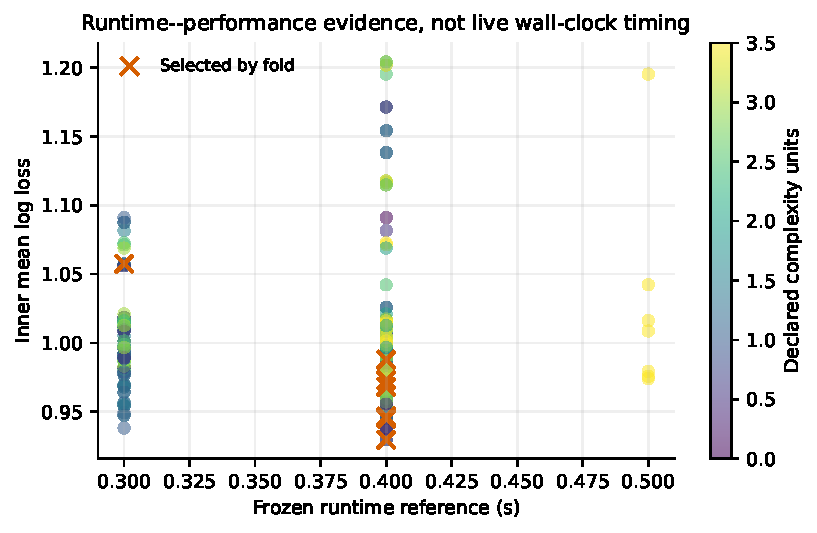
\includegraphics[width=\linewidth]{runtime_pareto.pdf}
\caption{Frozen runtime--performance evidence.}
\end{subfigure}\hfill
\begin{subfigure}{0.49\linewidth}
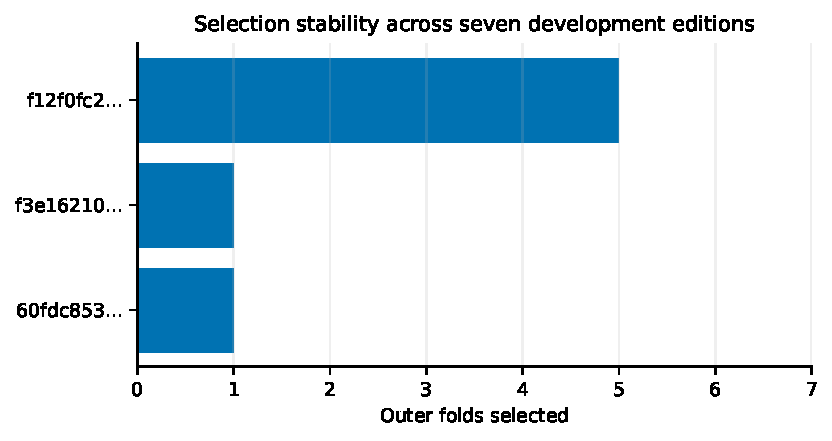
\includegraphics[width=\linewidth]{selection_stability.pdf}
\caption{Outer-fold selection frequencies.}
\end{subfigure}
\caption{Compute and stability diagnostics. Runtime values are pre-benchmarked references, not
live timing; the final candidate is modal in five of seven folds.}
\label{fig:selection}
\end{figure}

\begin{table}[htbp]
\centering
\caption{Equal-edition mean performance on the seven 1986--2010 outer folds.  Lower is better for
all loss columns; draw recall is secondary.  These are development OOF results, not 2014 results.}
\label{tab:benchmark}
\begin{tabularx}{\linewidth}{@{}Yrrrrr@{}}
\toprule
Model & WDL LL & Brier & Score NLL & Goal CRPS & Draw recall \\
\midrule
Advanced (nested calibrated) & 0.955 & 0.565 & 2.804 & 0.889 & 0.010 \\
Advanced (raw) & 0.955 & 0.565 & 2.804 & 0.889 & 0.000 \\
Independent mirrored Poisson & 0.984 & 0.584 & 2.825 & 0.876 & 0.000 \\
Legacy mirrored Dixon--Coles & 0.975 & 0.578 & 2.812 & 0.877 & 0.000 \\
Official multinomial logit & 0.991 & 0.589 & -- & -- & 0.000 \\
\bottomrule
\end{tabularx}

\end{table}

The calibrated advanced model has the best mean WDL log loss (0.9548) and Brier score (0.5646) in
\cref{tab:benchmark}.  Its draw recall under ordinary argmax remains essentially collapsed
(0.0095), so the probability result cannot support a claim of solved three-class decisions.  The
independent and legacy count baselines have better mean total-goal CRPS than the advanced model.

\begin{table}[htbp]
\centering
\caption{Paired advanced-minus-legacy differences.  The interval resamples tournament editions;
negative favors the advanced model.}
\label{tab:paired}
\begin{tabularx}{\linewidth}{@{}Yrrr@{}}
\toprule
Metric & Mean $\Delta$ & 95\% edition-bootstrap CI & Fold wins \\
\midrule
WDL log loss & -0.020 & [-0.037, -0.003] & 5/7 \\
Multiclass Brier & -0.013 & [-0.024, -0.003] & 5/7 \\
Scoreline NLL & -0.008 & [-0.028, +0.011] & 5/7 \\
Total-goal CRPS & +0.012 & [-0.008, +0.035] & 4/7 \\
\bottomrule
\end{tabularx}

\end{table}

\begin{figure}[htbp]
\centering
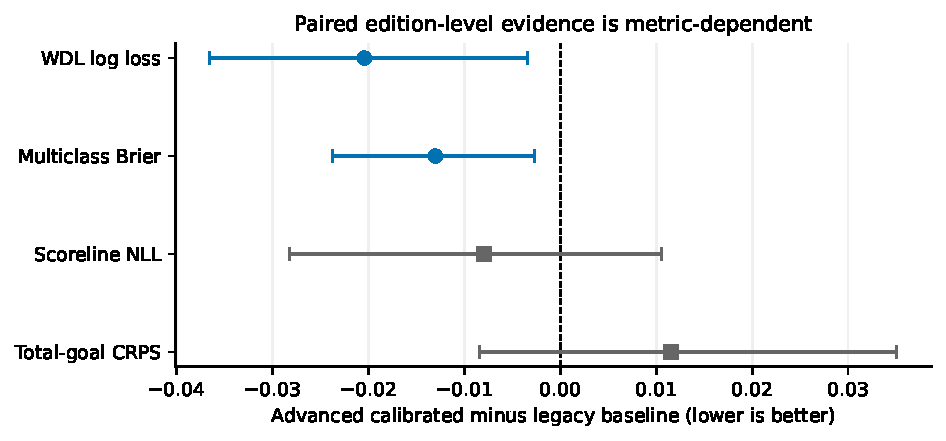
\includegraphics[width=0.93\linewidth]{paired_metrics.pdf}
\caption{The two WDL intervals lie below zero, whereas scoreline NLL and total-goal CRPS remain
inconclusive.  The CRPS point estimate is adverse.  The figure prevents a WDL result from being
over-generalized to the full joint distribution.}
\label{fig:paired}
\end{figure}

\begin{figure}[htbp]
\centering
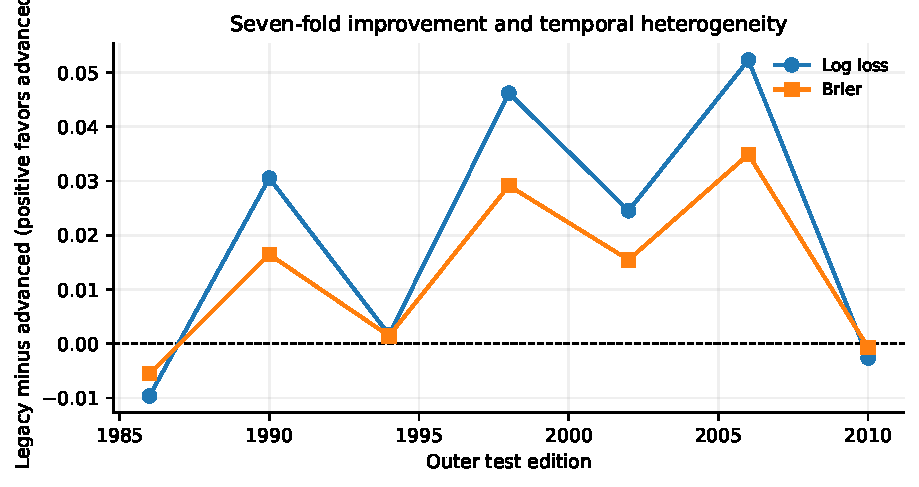
\includegraphics[width=0.88\linewidth]{fold_improvement.pdf}
\caption{Edition-specific legacy-minus-advanced improvements.  The two adverse 1986 values and
the variation across folds prevent a claim of uniform dominance or stationary effect size.}
\label{fig:fold-improvement}
\end{figure}

Relative to legacy Dixon--Coles, WDL log loss improves by $-0.02042$ and Brier by $-0.01302$ on
average, with both intervals below zero and five of seven edition wins
(\cref{tab:paired,fig:paired}).  Scoreline NLL also wins five folds but its interval
$[-0.02823,0.01052]$ crosses zero.  Total-goal CRPS wins four folds yet is worse by $0.01155$ on
average, with interval $[-0.00838,0.03507]$.  Fold wins alone therefore do not determine the claim.

\subsection{Calibration and the draw-aware action layer}

Nested calibration is selected as identity in three folds, temperature scaling in three, and
log-probability logit in one.  Relative to the raw advanced predictions, calibration worsens mean
log loss by $0.000262$ but improves Brier by $0.000221$.  This is a mixed near-zero result, not a
uniform calibration success.

\begin{figure}[htbp]
\centering
\begin{subfigure}{0.48\linewidth}
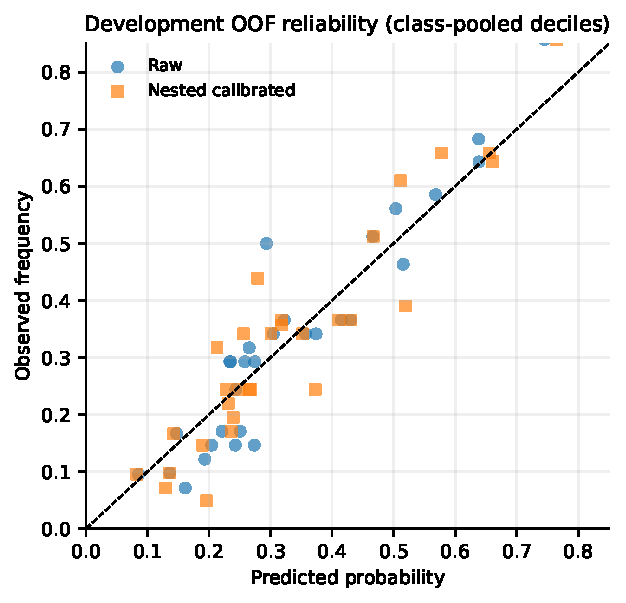
\includegraphics[width=\linewidth]{calibration_curve.pdf}
\caption{Class-pooled OOF reliability.}
\end{subfigure}\hfill
\begin{subfigure}{0.48\linewidth}
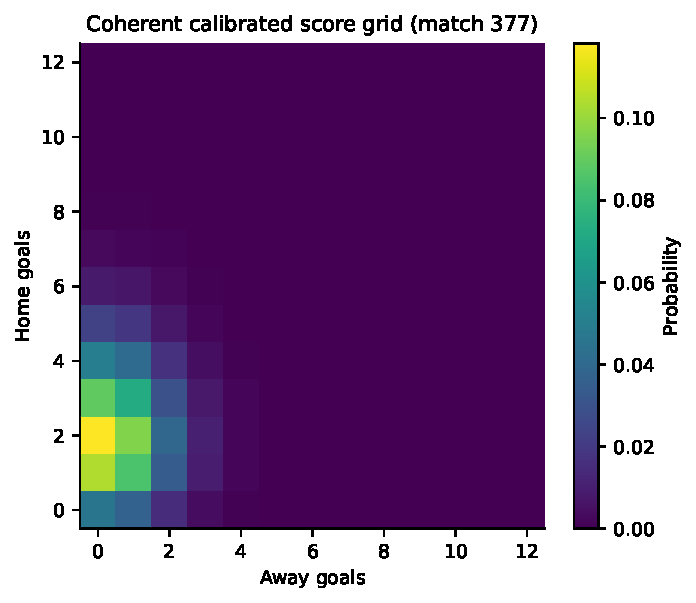
\includegraphics[width=\linewidth]{joint_score_heatmap.pdf}
\caption{One manifest-bound joint score grid.}
\end{subfigure}
\caption{Probability diagnostics.  Calibration is mixed, while the score heatmap illustrates the
coherent joint distribution whose WDL margins are recovered by partition projection.}
\label{fig:probability-diagnostics}
\end{figure}

The separate action layer produces at least one draw prediction in all seven folds and improves
macro-F1 in all seven, with mean macro-F1 gain $0.0944$ and mean draw recall $0.5137$.  Mean accuracy
falls by $0.0221$.  Probabilities are byte-for-byte unchanged.  We therefore retain a bounded
decision-theoretic conclusion---draw-sensitive utility changes useful actions---while rejecting the
stronger claim that the probability model itself ``solves draws.''

\subsection{A0--A8: what the full system rejects}

\begin{table}[htbp]
\centering
\caption{Ablation means over 14 edition--seed cells.  Negative values favor removing the component.
A4/A5 are measured zero effects because those components were inactive in A0; A8 is structurally
ineligible.}
\label{tab:ablation}
\begin{tabularx}{\linewidth}{@{}llrrY@{}}
\toprule
ID & Removed component & $\Delta$LL & $\Delta$Brier & Evidence decision \\
\midrule
A0 & none\_full\_model & +0.000 & +0.000 & Reference configuration. \\
A1 & dynamic\_ratings & +0.001 & +0.001 & Dynamic-state removal is small and unstable across editions. \\
A2 & player\_features & -0.003 & -0.000 & Removing player features improves the mean; no retained player-value claim. \\
A3 & era\_effects & -0.002 & -0.001 & Removing era effects improves the mean; no retained era-benefit claim. \\
A4 & correlated\_count\_model & +0.000 & +0.000 & Exact zero: the selected A0 model had no correlated-count component. \\
A5 & machine\_learning\_residual & +0.000 & +0.000 & Exact zero: the selected A0 model had no residual learner. \\
A6 & probability\_calibration & -0.000 & +0.000 & Calibration has mixed, near-zero aggregate effects. \\
A7 & hierarchical\_shrinkage & +0.149 & +0.049 & Zero team-effect penalty is much worse; shrinkage is essential here. \\
A8 & symmetry\_constraint & +0.046 & +0.030 & Structurally ineligible diagnostic. Asymmetric diagnostic degrades scores and violates the structural contract. \\
\bottomrule
\end{tabularx}

\end{table}

\begin{figure}[htbp]
\centering
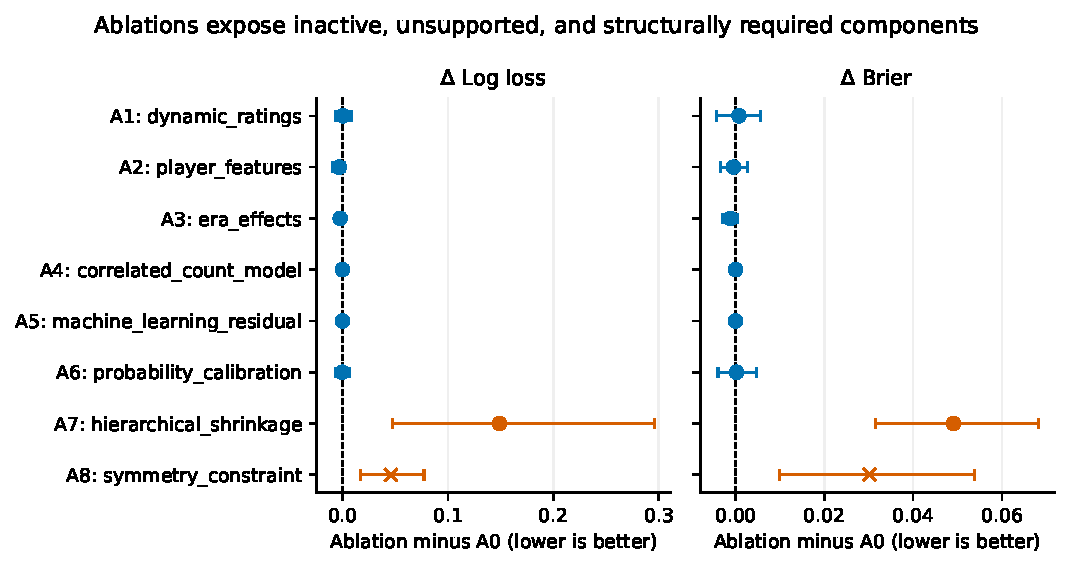
\includegraphics[width=\linewidth]{ablation_effects.pdf}
\caption{Edition-cluster intervals for A1--A8.  The cross marks A8, whose symmetry violation makes
it ineligible regardless of score.  A7 is the only large eligible degradation.}
\label{fig:ablation}
\end{figure}

The ablations overturn several intuitive claims (\cref{tab:ablation,fig:ablation}).  Removing the
available player block improves mean log loss by $0.00311$; removing the era encoding improves it by
$0.00215$.  These results reject the implemented representations, not every possible player or era
model.  The selected A0 specification already excludes shared-score dependence and residual ML, so
A4/A5 are exact zero-by-design measurements.  Removing calibration is mixed.  In contrast, setting
the team-effect penalty exactly to zero while retaining identified constraints and the context
penalty worsens log loss by $0.14894$ and Brier by $0.04911$; partial pooling is indispensable in
this sparse environment.  A8 reaches empirical swap error $0.47083$ and worsens log loss by
$0.04583$, supporting symmetry both as a validity condition and as useful inductive bias.

\subsection{Stress, historical transport, and safe refusal}

\begin{table}[htbp]
\centering
\caption{Measured robustness evidence and its claim boundary.}
\label{tab:robustness}
\begin{tabularx}{\linewidth}{@{}lY Y@{}}
\toprule
Check & Measured result & Claim boundary \\
\midrule
Structural stress matrix & 24 rows; 12 scenarios; all passed & Invariant checks, not predictive accuracy. \\
Swap/simplex errors & max 1.67e-16 / 2.22e-16 & Numerical structural certificate. \\
Extreme support & safe refusal at score support 60 & Abstention, not a valid extreme forecast. \\
All five format changes & MAE 27.53 direct vs 27.82 offset & Mixed historical pseudo-transport result. \\
Three team-field expansions & MAE 39.50 direct vs 23.45 offset; 3/3 wins & Historical subgroup; not a 2026 guarantee. \\
\bottomrule
\end{tabularx}

\end{table}

All 24 stress rows pass their declared structural verdicts; maximum symmetry and simplex errors are
$1.67\times10^{-16}$ and $2.22\times10^{-16}$.  These are numerical certificates.  A deliberately
extreme feature vector drives a fitted rate as high as 459.6; score support 60 retains insufficient
mass, and the system raises a \texttt{RuntimeError}.  This is successful safe refusal, not an
extreme-match prediction.

Historical pseudo-transport is conditional.  Across all five format changes, direct-total MAE is
27.53 and match-volume-offset MAE is 27.82, so the proposed separation does not win globally.  On
the predeclared three changes that also expand the team field, offset MAE is 23.45 versus 39.50 and
wins all three.  This subgroup result motivates, but cannot validate, expanded-format transport.

\begin{figure}[htbp]
\centering
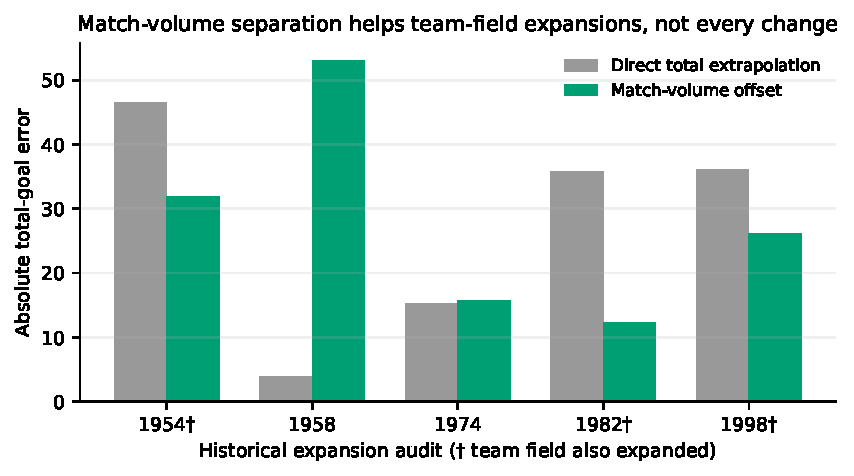
\includegraphics[width=0.92\linewidth]{format_transport.pdf}
\caption{Absolute error in five historical format-change audits.  The offset method helps all
three team-field expansions (dagger) but fails badly in 1958 and slightly in 1974.}
\label{fig:transport}
\end{figure}

The fixed edition-weight KL sensitivity preserves the advanced-versus-legacy WDL ordering at
$\epsilon=0.2$: robust log-loss risks are 0.9914 and 1.0048, respectively.  The weights increasingly
emphasize difficult editions, especially 2010, but the values are historical stress functionals,
not future error bounds.

\subsection{Parameter sensitivity and the replacement 2026-format scenario}

Whole-edition parameter bootstrap succeeds in 200/200 refits.  Across eight declared pre-2014
profile probes, the maximum class-probability standard deviation is 0.0507.  This is finite-probe
sensitivity, not predictive coverage.

The superseded tournament engine is still excluded because it paired adjacent qualifiers rather
than implementing Annex C.  Its numbers are not repaired or reinterpreted.  A replacement engine
independently implements all 495 third-place mappings and M73--M104, passes the 14 promotion checks,
and is linked to the final fit and Regulations hashes \citep{fifa2026regulations}.

\begin{table}[htbp]
\centering
\caption{Promoted replacement 2026-format scenario.  Historical team labels are profile stand-ins,
not a factual list of 2026 entrants.}
\label{tab:scenario}
\begin{tabularx}{\linewidth}{@{}lY Y@{}}
\toprule
Check & Measured result & Claim boundary \\
\midrule
Replacement simulation & 220,000 tournaments; adaptive MCSE thresholds met & Illustrative format scenario, not a factual entrant forecast. \\
Monte Carlo precision & max advancement/champion MCSE 0.0011 / 0.0010 & Predeclared adaptive thresholds or maximum-run termination. \\
Highest illustrative champion probability & BRA: 0.326 & Scenario-team labels are frozen model-transport profiles. \\
Expected tournament goals & 181.17 (MCSE 0.029) & 104-match official-format engine. \\
\bottomrule
\end{tabularx}

\end{table}

The adaptive run stops after 220,000 tournaments, the first batch at which maximum advancement and
champion MCSE are below 0.002 and 0.001.  The 104-match expected total is 181.165 (MCSE 0.0287).
These are conditional mechanics-and-transport quantities, not real-team forecasts.

\begin{figure}[htbp]
\centering
\begin{subfigure}{0.55\linewidth}
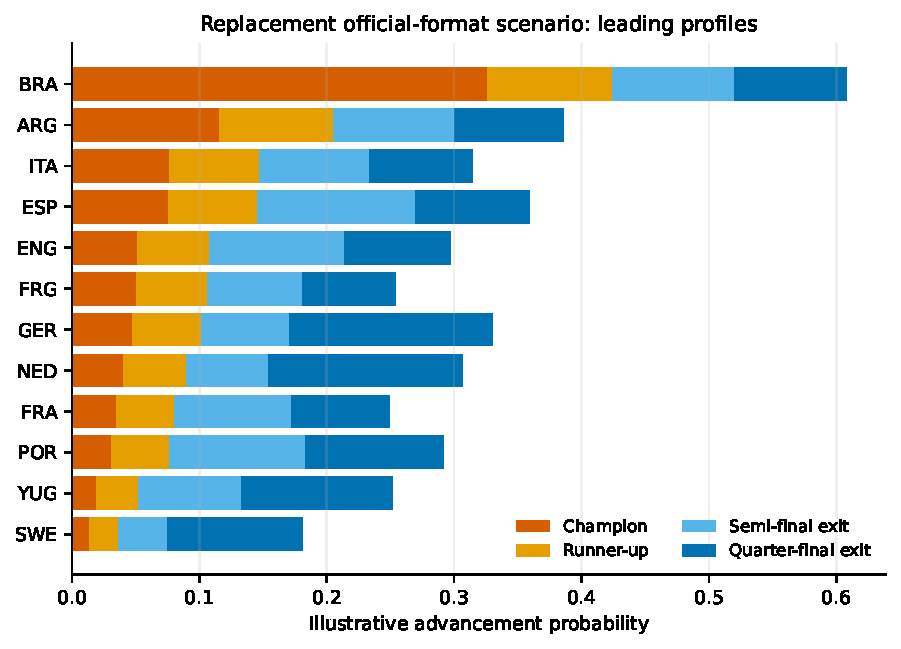
\includegraphics[width=\linewidth]{scenario_advancement.pdf}
\caption{Illustrative advancement profiles.}
\end{subfigure}\hfill
\begin{subfigure}{0.42\linewidth}
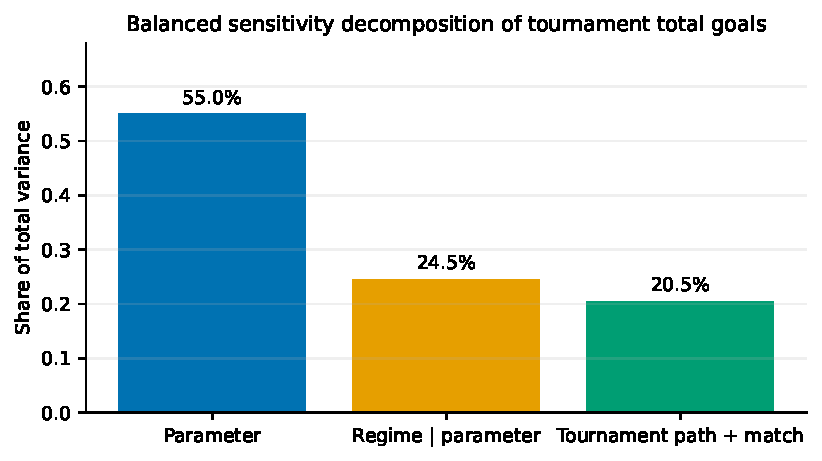
\includegraphics[width=\linewidth]{uncertainty_decomposition.pdf}
\caption{Balanced variance shares.}
\end{subfigure}
\caption{Replacement scenario evidence. Parameter, regime-given-parameter, and path-plus-match
components explain 55.0\%, 24.5\%, and 20.5\% of total-goal variance.  The decomposition is a
sensitivity identity, not a future coverage guarantee.}
\label{fig:scenario}
\end{figure}

\FloatBarrier
\section{One-Shot 2014 External Audit}

The promotion certificate was issued before any formal target access.  Phase 1 sealed outcome
probabilities and complete joint score grids for all 64 realized fixtures using team state frozen
before 2014.  Only then did phase 2 load a minimal truth table.  The result certificate records one
target read, no reopened selection, and cached-only repeats.  The estimand is batch-blind prediction
on the realized fixture set; it is not a prospective bracket forecast and not researcher blindness.

\begin{table}[htbp]
\centering
\caption{One-shot 2014 audit.  Losses are proper-score results; the cost-sensitive decision row has
no applicable probability score and is shown only for its action metrics.}
\label{tab:audit-2014}
\begin{tabularx}{\linewidth}{@{}Yrrrrr@{}}
\toprule
Model & WDL LL & Brier & Accuracy & Macro-F1 & Draw recall \\
\midrule
Advanced (frozen raw) & 1.023 & 0.609 & 0.531 & 0.389 & 0.000 \\
Advanced (frozen calibrated) & 1.023 & 0.609 & 0.531 & 0.389 & 0.000 \\
Official multinomial logit & 0.993 & 0.592 & 0.531 & 0.389 & 0.000 \\
Independent mirrored Poisson & 0.988 & 0.588 & 0.531 & 0.389 & 0.000 \\
Legacy mirrored Dixon--Coles & 0.985 & 0.588 & 0.547 & 0.399 & 0.000 \\
Advanced cost-sensitive decision & -- & -- & 0.422 & 0.404 & 0.385 \\
\bottomrule
\end{tabularx}

\end{table}

\begin{figure}[htbp]
\centering
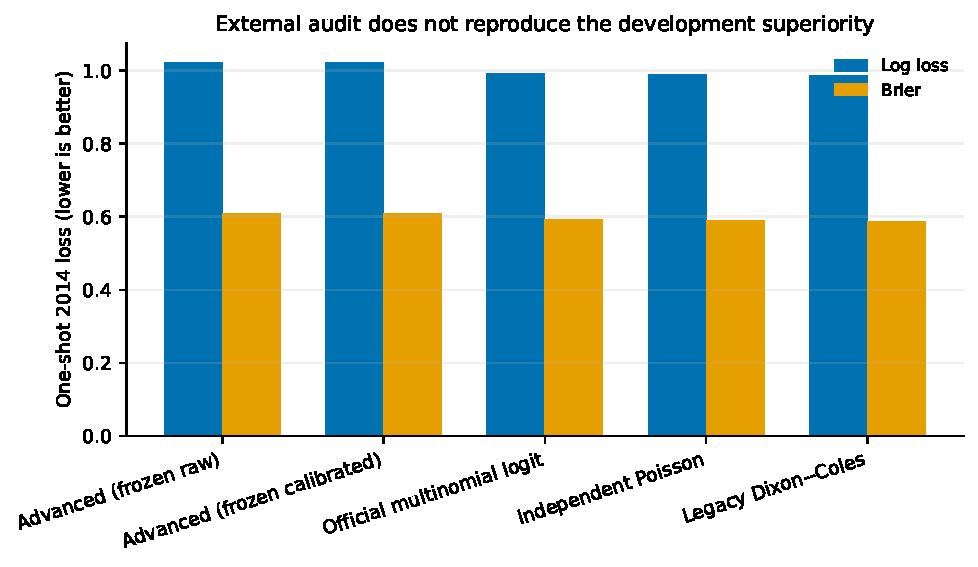
\includegraphics[width=0.92\linewidth]{audit_2014_comparison.pdf}
\caption{The external audit reverses the development WDL ordering.  This adverse result is retained
and does not trigger model reselection.}
\label{fig:audit-2014}
\end{figure}

The calibrated advanced model records log loss 1.0227 and Brier 0.6090, worse than frozen
Dixon--Coles at 0.9851 and 0.5876.  Accuracy is 0.5313 versus 0.5469.  Calibration is likewise worse
(0.1128 versus 0.0663), and the advanced scoreline NLL/total-goal CRPS are 3.1782/1.0300 versus
3.0236/0.9782.  The probability model predicts no draws by argmax.  The separately frozen
cost-sensitive action produces 26 draw decisions, draw recall 0.3846, and macro-F1 0.4038, at lower
accuracy 0.4219; proper scores are deliberately inapplicable to this action-only row.  Therefore the
defensible conclusion is development improvement without external superiority.

\section{Contribution Audit, Limitations, and Open Problems}

\subsection{What is substantively new here}

No isolated ingredient is presented as a field-first invention.  Joint Poisson scores, low-score
correction, dynamic strength, partial pooling, player ratings, calibration, model cards,
and dataset documentation have clear prior art
\citep{dixoncoles1997,ruesalvesen2000,baioblangiardo2010,mitchell2019,gebru2021}.  The defensible
contribution is an executable integration in which:

\begin{itemize}
  \item feature availability is a tested filtration contract rather than prose;
  \item even/odd representation and exact swap tests make exchange symmetry a model-eligibility
  rule;
  \item WDL calibration is reconciled to the score grid without changing within-partition odds;
  \item model choice, calibration, action utility, ablation, and uncertainty remain nested within
  earlier editions; and
  \item failures are promotion-relevant artifacts, including inactive components, adverse
  ablations, mixed proper scores, and explicit refusal outside score support.
\end{itemize}

This system-level contribution advances auditability and falsifiability.  It should not be inflated
into universal predictive superiority.

\subsection{Limitations and threats to validity}

\begin{enumerate}
  \item \textbf{Few independent environments.} Seven scored editions cannot identify small and
  heterogeneous effects with high precision.  Cluster intervals have only seven unique units.
  \item \textbf{Non-pristine human boundary.} The protocol precedes the complete advanced run, but
  investigators had seen legacy 2014 results and structural pilots.  Software isolation does not
  restore human blindness.
  \item \textbf{Model-family scope.} The selected family cannot rule out negative-dependence
  copulas, discontinuous state changes, or better residual learners.  A4's zero is selection-
  conditional.
  \item \textbf{Personnel semantics.} Player events are sparse, lineup availability is historically
  nonuniform, and the A2 result rejects only the available aggregate representation.
  \item \textbf{Historical target ambiguity.} Extra time, rule changes, and predecessor-state
  identity are imperfectly normalized.  Association is not causation.
  \item \textbf{Calibration sample size.} Inner cross-fitting sometimes compares methods on only one
  or two eligible editions; identity frequently wins.  Calibration error itself is noisy.
  \item \textbf{External audit.} The single 2014 edition has only 64 matches and uses a
  batch-blind realized-fixture information set.  It rejects external superiority but cannot by
  itself estimate a stable distribution of future-edition effects.
  \item \textbf{Uncertainty scope.} Whole-edition bootstrap and balanced tournament decomposition
  are sensitivity analyses, not guaranteed coverage under arbitrary institutional change.
  \item \textbf{2026 mechanism.} The replacement engine is graph-correct, but it uses historical
  profile stand-ins rather than factual 2026 entrants, qualification information, or future form.
\end{enumerate}

\subsection{High-value next falsifiers}

The next research stage should prioritize questions capable of overturning the present model:
\begin{enumerate}
  \item a negative-dependence-capable score family under the identical nested folds;
  \item change-point or state-space attack/defence dynamics;
  \item lineup-missingness-aware personnel models separated by issuance filtration;
  \item bracket-functional calibration evaluated on additional held-out historical tournaments;
  \item partial-identification envelopes for field-strength and scoring-regime shift; and
  \item factual entrant/profile updates performed without changing the frozen mechanics engine.
\end{enumerate}
Any follow-on model must be a new version; the completed 2014 audit cannot be reused for selection.

\section{Reproducibility, Governance, and Disclosure}

The paper tables and figures are regenerated only from \path{temp/advanced_evidence} by
\path{scripts/build_paper_artifacts.py}.  The builder fails closed unless development evidence ends
at 2010, the promotion certificate revalidates, and the one-shot audit verifies as target-read once,
selection-closed, and cached-only.  It loads only the promoted replacement simulation and
lineage-bound decomposition.  \path{doc/artifact_manifest.json} records SHA-256 values for every
admissible source and 33 generated artifacts, plus the superseded-evidence ledger.
\path{doc/tables/paper_evidence.json} is the bridge between prose and numbers.  Exact protocol,
data, and selected-model hashes are:

\begin{itemize}
  \item protocol: \nolinkurl{8b3148e65846383a767ae20e98f863a457d7f914f71ef73a31e9b988d37b06f3};
  \item deviation record: \nolinkurl{6f487cf1331d45e2591bcc905444bb2f1214481d2fab7a5c3c3c47f40e75cf0c};
  \item development frame: \nolinkurl{23eba94cf43c6773cad691e66704022442683169311b7c9b5a09ca9817216451};
  \item feature schema: \nolinkurl{f5db6b9a447b6300bf466673cda9fa4e0265bc13c1ab2c81d44a0e63b3fdb9cc};
  \item selected configuration: \nolinkurl{77ba14cb38a364b145be15ec4474811bc6bd0914452e438d34d415ee604c366b};
  \item final fit: \nolinkurl{10238a4c6d368e50acb9ac28e4523dbd1b4f1b64710667ba0e8eb511b8774f53}.
\end{itemize}

Bibliographic identities and bounded source claims were separately screened in a 58-row citation
audit.  Post-2014 methods may motivate analysis but never supply closed-track outcomes or features.
The data are intended for retrospective competition research, not betting, causal player
evaluation, or high-stakes decisions.  An AI coding/research assistant was used for code drafting,
artifact generation, and manuscript organization; all quantitative statements are bound to the
executable evidence files, and no AI-generated statement substitutes for the audit certificates.

\section{Conclusion}

The development evidence supports a bounded WDL proper-score improvement, but the one-shot 2014
audit does not reproduce it and therefore rejects a claim of external superiority.  This is the
central empirical result, not a footnote.  Player and era encodings do not survive ablation, shared
dependence and residual ML are not selected, calibration is mixed, and total-goal CRPS is adverse
both in development mean and in the audit.  Team-effect shrinkage and exchange symmetry remain
important within the implemented family.  A corrected official-format engine supports a bounded
220,000-run 2026 mechanics scenario and sensitivity decomposition, not a factual entrant forecast.
The scientific contribution is the evidence discipline that makes all three conclusions coexist
without selection leakage or post-hoc model rescue.

\section*{Data and Code Availability}

The repository contains the immutable competition inputs, protocol lock, data/model cards, source
audit, frozen development evidence, manuscript builder, tables, figures, and artifact manifest.
Rebuild commands and exact verification points are listed in \texttt{RESEARCH\_REPORT.md}.

\bibliographystyle{plainnat}
\bibliography{references}

\appendix
\small
\section{Exact Evidence Refresh Points}

The one-shot 2014 audit is complete and may only be cache-verified; it must not be regenerated after
seeing its targets.  For this frozen version, the minimum refresh chain is:
\begin{enumerate}
  \item verify the protocol/deviation locks, frozen identity, and all seven pre-audit manifests;
  \item verify the promotion certificate and cached audit certificate with target reads fixed at one;
  \item verify the official Annex C/M73--M104 simulation and decomposition lineage;
  \item run \texttt{uv run python scripts/build\_paper\_artifacts.py};
  \item run the paper-artifact tests and citation resolver; and
  \item compile with XeLaTeX/BibTeX and inspect the rendered pages.
\end{enumerate}

\section{Interpretation Rules for Reviewers}

\begin{itemize}
  \item Every reported difference is candidate minus baseline or ablation minus A0; lower losses
  are better.  A8's score remains secondary to its structural ineligibility.
  \item Edition-bootstrap intervals quantify resampling variation across seven historical
  environments; they are not seven-independent-study meta-analysis intervals.
  \item A4/A5 are zero because A0 lacks those selected components, not because the scientific
  concept is universally valueless.
  \item Former wrong-graph scenario totals remain withdrawn; only the manifest-bound replacement
  scenario may be quoted, and only as historical-profile mechanics sensitivity.
  \item The 2014 table is an external audit and cannot be folded back into model selection or pooled
  with the seven development editions.
\end{itemize}

\end{document}
